%Redefinir Requesitos
%Mudar Introdução
%Especificar Detalhaes dos Requesitos
%Gestão de Conflitos entre Alex e Pedro (gestores)
%Modelo Descentralizado
%Recursos de Hardware e Software
%Conclusão do COCOMO
%Divisão de Tarefas GANT
%Organização GANT
%Riscos Muito Genericos ESPECIFICAR
%PLANO FMAMN Definir fail safes para os riscos que acontecerem
%Razoavelzinho :(





%formatação do documento e tipo do documento
\documentclass[12pt, a4paper, twoside]{report} %inicio do doc

%pacotes de extensões
\usepackage[portuges]{babel} %pkg da lingua portugues
\usepackage[latin1,utf8]{inputenc} %pkg da lingua portugues
\usepackage{verbatim} %pkg para escrever sem formataçao
\usepackage{color} %usar cores nas letras
\usepackage{graphicx} %usar imagens no doc
\usepackage[table,xcdraw]{xcolor}
\usepackage{makeidx}
\usepackage{anysize} % para formatar o tamanho do documento
\usepackage{multirow}
\usepackage{mathtools}
\usepackage{wrapfig}
\usepackage{footnote}

\marginsize{3.17cm}{3.17cm}{2.54cm}{2.54cm}

%fazer índice
\makeindex

\begin{document}

\title{%
	\textbf{Planeamento e Gestão de Projecto}\\ 
	\large Relatório Fase 2
}

\author{%
Alexandre Machado, nº 43551 \\
Nuno Silva, nº 44285 \\
Francisco Pires, nº 44314 \\
}

\date{\today}
\maketitle
\tableofcontents

%--------------------------------------------------------------------------------------------- Feito

\chapter{Introdução}

\textit{Foram feitas alterações nas partes entregues na primeira fase.} \\


Este projecto tem como objectivo o desenvolvimento e a implementação de um Sistema de Informação (SI), dirigido aos utentes do Serviço Nacional de Saúde (SNS). 
Este SI é baseado em tecnologias \textit{web} e pretende melhorar a qualidade dos serviços prestados ao utilizador. 
Após a consulta do Portal da Saúde, e a identificação das capacidades existentes, propomos ampliar os requisitos funcionais disponíveis para o utilizador e melhorar os requisitos não funcionais. 
Para isso, pretendemos assegurar a melhor disponibilidade dos servidores, correcções na interface do \textit{website} e confidencialidade dos dados associados ao utilizador.

%--------------------------------------------------------------------------------------------- Feito

\chapter{Análise de requisitos}

\section{Requisitos funcionais e não funcionais}

\subsection{Requisitos funcionais}

De acordo com os objectivos definidos para este projecto, selecionamos as seguintes funcionalidades que o utilizador terá disponíveis neste SI.

\begin{itemize}

\item Registo de contactos e dados pessoais
\begin{itemize}
\item Nº do Cartão de Cidadão, Nº de Utente de Saude, Nº de telefone, NIF, Email.
\end{itemize}
\item Definir agregado familiar
\begin{itemize}
\item Pai, mãe, filhos, irmãos, etc...
\end{itemize} 
\item Identificação de cuidador familiar
\item Registo de informação pessoal relevante
\begin{itemize}
\item Testamento Vital, Contados de emergência
\end{itemize}
\item Registo de indicadores básicos de saúde
\begin{itemize}
\item Medicação, alergias, diagnósticos, cirurgias, vacinação, doenças raras
\end{itemize}
\item Registo de exames complementares de diagnóstico
\begin{itemize}
\item Todo o tipo de exames(documentos relevantes) que o utente faça podem ser guardados
\end{itemize}
\item Consulta de registos clínicos
\item Pedido de prescrição de medicação crónica
\item Marcação de consultas
\item Inscrição e consulta das listas para cirurgia (eSIGIC)
\item Definir estado no Registo Nacional de Não Dadores (RENNDA)
\item Pesquisa de serviços médicos (directório)
\begin{itemize}
\item Poder pesquisar serviços médicos por área
\end{itemize}
\item Pedido de mudança de médico de família
\item Pedido de isenção de taxas moderadoras

\end{itemize}

%--------------------------------------------------------------------------------------------- Feito

\subsection{Requisitos não funcionais}

Para execução das funcionalidades neste SI, será necessário assegurar os requisitos não funcionais que listamos de seguida.

\begin{itemize}
\item Confidencialidade dos dados
\begin{itemize}
\item Todos os dados médicos que o utente introduz na plataforma, este pode escolher que informação pode partilhar com o medico
\end{itemize}
\item Segurança dos dados e dos acessos
\begin{itemize}
\item Os dados introduzidos são salvagardados de qualquer tipo de intrusão ou acesso não autorizado
\end{itemize}
\item Garantia de disponibilidade
\begin{itemize}
\item Garantir que a plataforma está sempre acessível online (24/7)
\end{itemize}
\item Escalável e modular
\begin{itemize}
\item Capacidade de poder aumentar a capacidade de servir um maior numero de clientes
\end{itemize}
\item Tempo de resposta
\begin{itemize}
\item A plataforma terá um tempo de resposta o mais imediato possível
\end{itemize}
\item Assegurar o cumprimentos das normas legais
\item Resolução de conflitos
\begin{itemize}
\item Garantir que a informação que o utente e o medico introduzem não divergem
\end{itemize}
\item Persistência e sincronização dos dados
\begin{itemize}
\item A informação ser partilhada entre servidores de maneira a garantir não haver falhas de dados
\end{itemize}
\item Notificações e alertas de acontecimentos do utilizador
\begin{itemize}
\item Estas serão enviadas para o utente ou o medico via email ou telemóvel
\end{itemize}
\item \textit {Responsive Web Design}
\end{itemize}

%--------------------------------------------------------------------------------------------- Feito

\chapter{Planeamento}

\section{Recursos}

\textbf{Recursos Humanos}
\\

Os recursos humanos para o projecto incluem seis alunos de Tecnologias de Informação (LTI), sendo que os três alunos não presentes neste relatório pertencem ao grupo 003. 
No final da cadeira de Planeamento e Gestão do Projecto (PGP), os dois grupos irão juntar-se e trabalhar em conjunto nas cadeiras de Projecto Tecnologias de Informação (PTI) e Projecto Tecnologias de Redes (PTR). A duração total do projecto será de sete meses, sendo três meses e meio dedicados ao planeamento (PGP).
\\
\\
\textbf{Disponibilidade}
\\

A disponibilidade dos alunos é conforme apresentada na seguinte tabela:

\begin{table}[h]
\centering
\begin{tabular}{|l|c c|}
\hline
\multirow{2}{*}{} & \multicolumn{2}{c|}{Disponibilidade} \\ \cline{2-3} 
                  		& 1ºSemestre        & 2ºSemestre       \\ \hline
Pedro Neves       		& 20\%              & 40\%             \\ \hline
Rita Capela       		& 20\%              & 28,6\%           \\ \hline
Tiago Maurício    		& 20\%              & 28,6\%           \\ \hline
Francisco Pires   		& 20\%              & 33,3\%           \\ \hline
Alexandre Machado 		& 20\%              & 28,6\%           \\ \hline
Nuno Silva\footnotemark	& 10\%              & *                \\ \hline
\end{tabular}
\caption{Tabela de Disponibilidade}
\label{disponibilidade}
\end{table}

\footnotetext{ O aluno em questão encontra-se a trabalhar em \textit{part-time}, pelo que no primeiro semestre tem menos disponibilidade. Não sendo possível prever, por agora, a sua disponibilidade no segundo semestre, foi decidido não ser calculada.}

\clearpage

%---------------------------------------------------------------------------------------------

\noindent{\textbf{Organização da equipa}}
\\
\\
A organização dos membros envolvidos vai ser feita em três grupos.
Um grupo para PTR, um para PTI, e um ultimo grupo para os \textit {"elementos moveis"}. 
Estes alunos vão contribuir em conjunto para o trabalho de ambas as cadeiras, e ao mesmo tempo, gerir o funcionamento e as decisões dos grupos.
A decisão de organizar o projecto distribuído em três grupos surgiu para dar resposta ao facto de dois membros terem competências equivalentes em PTI e PTR e disponibilidade acrescida para gerir o projecto no seu conjunto.

\begin{itemize}
\item Grupo PTR
\begin{itemize}
	\item Francisco Pires
	\item Nuno Silva
\end{itemize}
\item Grupo PTI
\begin{itemize}
	\item Tiago Maurício
	\item Rita Capela
\end{itemize}
\item \textit{Elementos Moveis}
\begin{itemize}
	\item Alexandre Machado
	\item Pedro Neves
\end{itemize}
\end{itemize}

\noindent{\textbf{Tabela de Competências}}
%COMPLETAR AS COLUNAS DE DESIGN E RH
\begin{table}[h]
\centering
\begin{tabular}{|l|c c c c c c c c c|}
\hline
                  & PHP & Java & HTML & CSS & Python & Interface & Gestão  & Design & RH\\ \hline
Pedro Neves       & 3   & 4    & 3    & 2   & 4      & 1         & 4       & ?      & ?     \\ \hline
Rita Capela       & 3   & 2    & 4    & 4   & 3      & 4         & 4       & ?      & ?     \\ \hline
Tiago Maurício    & 3   & 4    & 4    & 3   & 4      & 2         & 3       & ?      & ?     \\ \hline
Francisco Pires   & 2   & 3    & 4    & 3   & 4      & 3         & 3       & ?      & ?     \\ \hline
Alexandre Machado & 2   & 4    & 4    & 4   & 4      & 3         & 4       & 3      & ?     \\ \hline
Nuno Silva        & 2   & 4    & 4    & 4   & 4      & 3         & 3       & ?      & ?     \\ \hline
\end{tabular}
\caption{Tabela de Competências}
\label{competencias}
\end{table}

\clearpage

%---------------------------------------------------------------------------------------------

\section{Estimação}

Para a realização da tabela relativa aos dados históricos, foram escolhidas as cadeiras em que a matéria dos projectos se encaixa no âmbito do projecto.

\begin{table}[h]
\centering
\begin{tabular}{|l|c c c c c|}
\hline
                  & AD        & ASW       & ITW     & ADS     & SO      \\ \hline
Alexandre Machado & 1002/160h & 2576/160h & 756/72h & 454/18h & 560/42h \\ \hline
Francisco Pires   & 1002/160h & NA        & 687/5h  & NA      & 775/50h \\ \hline
Nuno Silva        & 942/150h  & NA        & 542/10h & 500/35h & 700/60h\\ \hline
\end{tabular}
\caption{ Dados Históricos (\textit{Lines of Code} e horas).}
\label{my-label}
\end{table}

\subsection{Esforço disponível}

\begin{itemize}

\item 1º semestre (duração: 3,5 meses)
\begin{equation}
20+20+20+20+20+10 = 110 \ (1,1 \ pessoas)
\end{equation}
\begin{equation}
E = 1,1 \ . \ 3,5 = 3,85 \ PM
\end{equation}
\item 2º semestre (duração: 3,5 meses)
\begin{equation}
40+28,6+28,6+33,3+28,6 = 188 \ (1,88 \ pessoas)\\
\end{equation}
\begin{equation}
\ E = 1,88 \ . \ 3,5 = 6, 58 \ PM
\end{equation}
\end{itemize}

\subsection{Linhas de código}

As linhas de código previstas para o projecto são conforme apresentadas na seguinte tabela:

\begin{savenotes}
\begin{table}[h]
\centering
\begin{tabular}{|l|c c c c|}
\hline
                       					& Optimista & Provável & Pessimista & \textbf{Final} \\ \hline
Criar a Base de Dados  					& 50        & 120      & 200        & 123   		 \\ \hline
Configurar \textit{HTTP Server} 		& 5         & 20       & 50         & 25    		 \\ \hline
Ligação à Base de Dados \footnote{Linhas a não serem consideradas usando a linguagem \textit{Java}.}
										& 5         & 10       & 20         & 12    		 \\ \hline
Segurança              					& 200       & 300      & 350        & 283   		 \\ \hline
Sistema Distribuído\footnotemark	    & 2000      & 3750     & 5000       & 3583   		 \\ \hline
\textit{Views}            				& 1000      & 1500     & 2500       & 1600  		 \\ \hline
Controlador                 			& 500       & 750      & 1000       & 750   		 \\ \hline
Modelo                      			& 200       & 300      & 500        & 333   		 \\ \hline
\textbf{Total}		   					& 3960      & 6750     & 9620       & \textbf{6777}  \\ \hline
\end{tabular}
\caption{Linhas de Código}
\label{codigo}
\end{table}%
\end{savenotes}

\footnotetext{Considera-se por SD a programação integral de um Sistema Distribuído. Caso se use um serviço que somente precise de configuração (p.ex. \textit{Amazon Web Services}), estas linhas devem ser alteradas.}

%---------------------------------------------------------------------------------------------

\subsection{Modelos Empíricos}

Calculo do esforço orgânico:
\\

\begin{equation}
E = a \ . \ KLOC ^ b
\end{equation}

\begin{equation} E = 2,4 \ \bigg({N.Linhas \over 1000}\bigg)^{1.05}
\end{equation}

\begin{equation}
{E = 2,4 \ \bigg({6777 \over 1000}\bigg) ^ {1.05}}
= 17.89 \ P.M
\end{equation}

Calculo da Duração:

\begin{equation}
D = c \ . \ E^d
\end{equation}

\begin{equation}
D = 2,5 \ (17,89)^{0,38}= 7,48\ M
\end{equation}
\\
\section{Processo de Desenvolvimento de Software}

Como processo de desenvolvimento do nosso projeto decidimos usar o Processo Unificado.
Esta decisão foi baseada numa reflexão da nossa parte, em que, pensámos na forma como trabalhamos e, visto que este projeto não é de forma alguma \textit{full-time}, tivemos de ter isso em conta. O Processo Unificado permite-nos avançar iterativamente e ao mesmo tempo voltar a trás sem que hajam muitos problemas, havendo assim um balanço entre o avançar no projeto e ajustar problemas anteriores, o que achamos que seria perfeito no nosso caso.
\\
%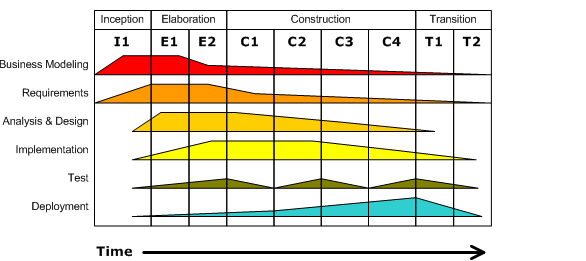
\includegraphics[scale=0.6]{image1.png}

\begin{figure}[h!]
  \centering
    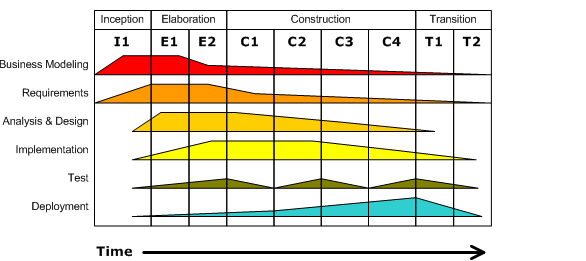
\includegraphics[width=0.6\textwidth]{image1.png}
   \caption{Exemplo de um Processo Unificado}
\end{figure}

\clearpage

\textbf{O Processo Unificado divide-se em quarto fases:}
\\

\begin{enumerate}
\item \textit{Inception} – justifica-se a execução do projeto, ou seja, tenta-se adquirir um conhecimento do que irá ser preciso para concluir o projeto e quando concluído, os resultados deste.

\item \textit{Elaboration} – conclui-se de certa forma a fase de \textit{inception}, visitando com mais detalhe todos os fatores de risco, \textit{reward} e recursos que este irá trazer. Convém ser o mais completo e detalhado possível visto que na fase seguinte vai proceder-se à construção do projecto.

\item \textit{Construction} – começa-se a construção do que irá ser uma versão operacional do projeto. O foco principal nesta fase é a construção de features discutidas anteriormente. É de valor notar que em projetos de maior dimensão esta fase poderá ter varias iterações.

\item \textit{Transition} – o foco nesta fase será transitar o projeto de um ambiente de desenvolvimento para um ambiente de produção, pondo o produto disponível ao cliente final, para que este o perceba e o use. Nesta fase faz-se o treino do cliente final e o beta testing para validar o projeto em relação às expectativas do cliente final. De seguida compara-se o estado do projeto nesta fase à fase de Inception e se tudo estiver bem, faz-se uma \textit{release}.

\end{enumerate}
%---------------------------------------------------------------------------------------------

\textbf{Vantagens do Processo Unificado:}
\begin{itemize}
\item O cliente não precisa de esperar muito tempo para entrar em contacto com um resultado prático.
\item Quando terminado o desenvolvimento do projeto é muito dificil encontrar erros dada a facilidade de os corrigir anteriormente.
\item Os riscos de grau mais elevado são trabalhados em primeiro lugar, dando assim alguma confiança no desenvolvimento do projeto
\end{itemize}

\textbf{Desvantagens do Processo Unificado:}
\begin{itemize}
\item Poderá haver desorganização em períodos mais avançados no projeto.
\item Aumento de gastos em implementações de varias versões do projetos.
\end{itemize}

%---------------------------------------------------------------------------------------------

\clearpage

%\section{Planeamento do Projecto}

\section{Gestão de Riscos}

Nesta avaliação dos riscos para o nosso projeto, identificámos que existem três grandes áreas: a de Relações Humanas, a de Tecnologia e a de Desenvolvimento do projeto.\\\\ Na categoria de RH identificámos que os principais problemas têm a haver com a relação entre membros do grupo e o comportamento de cada um. \\\\Consideramos estes riscos bastante importantes visto que uma má dinâmica de grupo pode arruinar o potencial de um projeto.\\\\ Na categoria de Tecnologia identificámos que bugs e a segurança são os principais riscos a ter em conta e, iremos dar ênfase à segurança no projeto, visto que uma das partes mais criticas é o tipo de informação que iremos tratar.\\\\ Por ultimo, na categoria de desenvolvimento do projeto, identificámos que, sem surpresa, o maior problema são os atrasos que poderão acontecer, podendo estragar planos e horários planeados para a completação do projeto.\\\\ Em geral achamos que os nossos riscos irão ser de natureza comum a todos os grupos, são riscos que a maioria dos projetos, quer a nível académico ou profissional, encontram, não significando que os podemos levar menos a serio, sendo esta a causa de projetos falhados em varias áreas.

\clearpage
\noindent\textbf{Riscos de RH:}
\\
\begin{itemize}
\item Má comunicação
\item Falta de empenho
\item Falta de conhecimento
\item Baixa de um membro do grupo
\item Falta de “química” entre membros do grupo
\item Atraso na entrega de trabal de um membro do grupo
\item Desistência de um membro do grupo
\end{itemize}
\textbf{Riscos de Tecnologia:}
\\
\begin{itemize}
\item Má implementação (bugs) de uma funcionalidades
\item Updates que pioram o funcionamento de funcionalidades
\item Falta de segurança do projetos
\end{itemize}
\textbf{Riscos no desenvolvimento do projeto:}
\\
\begin{itemize}
\item Atrasos na entrega do projeto
\item Falta de funcionalidades na entrega do projeto final
\item Requisitos incompletos
\end{itemize}

\clearpage

\noindent\textbf{Tabela de Riscos:}

\begin{enumerate}
\item Má comunicação
\item Falta de empenho    
\item Falta de conhecimento 
\item Baixa de um membro do grupo
\item Falta de “química” entre membros do grupo
\item Atraso de prazos internos 
\item Desistência de um membro do grupo
\item Má implementação (bugs) de uma funcionalidade 
\item Updates que pioram o funcionamento de funcionalidades
\item Falta de segurança na implementação 
\item Atrasos na entrega de etapas do projeto
\item Falta de funcionalidades na iteração final do projeto
\item Requisitos incompletos
\end{enumerate}

\begin{table}[h]
\centering
\begin{tabular}{|l|l l l|}
\hline
Riscos                              & Tipo             & Probabilidade & Impacto \\ \hline
1				                    & Recursos Humanos & Baixa         & 2       \\ \hline
2                               	& Recursos Humanos & Média         & 2       \\ \hline
3                                	& Recursos Humanos & Média         & 3       \\ \hline
4                          			& Recursos Humanos & Baixa         & 2       \\ \hline
5             						& Recursos Humanos & Média         & 3       \\ \hline
6                            		& Recursos Humanos & Média         & 2       \\ \hline
7                     				& Recursos Humanos & Baixa         & 3       \\ \hline
8        							& Tecnologia       & Elevada       & 2       \\ \hline
9 									& Tecnologia       & Baixa         & 2       \\ \hline
10                   				& Tecnologia       & Elevada       & 3       \\ \hline
11              					& Desenvolvimento  & Elevada       & 1       \\ \hline
12 									& Desenvolvimento  & Média         & 2       \\ \hline
13                                	& Desenvolvimento  & Baixa         & 1       \\ \hline
\end{tabular}
\caption{Tabela de Riscos}
\label{riscos}
\end{table}

%---------------------------------------------------------------------------------------------

\chapter{Conclusão}

Perante o projecto que nos foi proposto, definimos os requisitos funcionais e não funcionais como pilares da nossa proposta de trabalho. 
Através de uma pesquisa ao \textit {website} do Portal do Utente e um conjunto de boas práticas de serviços \textit {web}, adicionamos funcionalidades possíveis de implementar no SI, e que determinam uma melhoria, tanto no serviço, como na interacção com o utilizador.

%---------------------------------------------------------------------------------------------

\chapter{Bibliografia}

%\begin{thebiblography} {99}

\end{document}